\documentclass{article}
\usepackage{graphicx,wrapfig,lipsum}
\begin{document}

\title{\textbf{Journal 1}}
\author{Ahmed Al Guqhaiman}
\date{\today}
\maketitle

\begin{wrapfigure}{r}{1.5in}
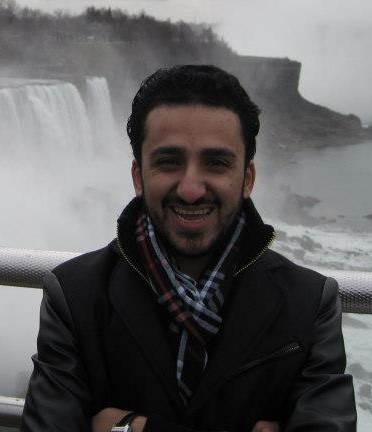
\includegraphics[width=1.5in]{Niagara_Falls.jpg}
\end{wrapfigure} 
{\lipsum[0-0]

The computer science research class is the first research course I have ever taken. Thus, it will be very helpful for me as a graduate student throughout my research journey. I hope to learn the most effective research methods for the most common computer science dissertations \cite{Yu2014}. Learning the differences between qualitative, quantitative, and mixed methods in details with the most effective tools in each approach are also critical. How to find and select the most suitable workshops, conferences, and journals is extremely important. I also would like to distinguish the good venues from the bad ones. Moreover, I need to learn how to read and write papers more effectively. In particular, I need to learn how to develop a thesis proposal, develop a hypothesis, define a good problem statement, collect and analyze data, find the appropriate data set, use the results to make a qualitative or quantitative conclusion, do statistical analysis, and present research paper more effectively. Investigating a problem can be done through questionnaires and interviews.\cite{Sharif-Yazd2017} In either approach, when the number of participants will be enough to generalize the results and be publishable in a good venue. In this type of research, I would also like to learn how to deal with the incomplete survey, combine data from multiple sources, analyze the survey data, collect data more effectively. At the end of this semester, I hope that my research paper meets the standard to get accepted for publication in a top rank conference. I am a Ph.D. student in the Engineering Security program. This year is my junior year and my research interests lie in the Media Access Control (MAC) protocols, routing protocols, Software Defined Network (SDN), and network security. I just became a father to a beautiful baby girl four months ago and named her Ledn.





\clearpage
\bibliographystyle{ieeetr}
\bibliography{Bibliography}





\end{document}
